\chapter{\IfLanguageName{dutch}{Stand van zaken}{State of the art}}%
\label{ch:stand-van-zaken}

% \begin{figure}
%   \centering
%   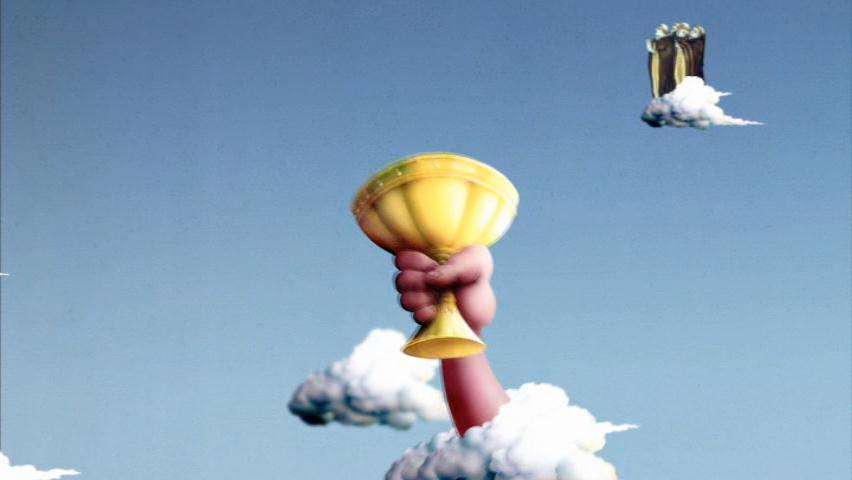
\includegraphics[width=0.8\textwidth]{grail.jpg}
%   \caption[Voorbeeld figuur.]{\label{fig:grail}Voorbeeld van invoegen van een figuur. Zorg altijd voor een uitgebreid bijschrift dat de figuur volledig beschrijft zonder in de tekst te moeten gaan zoeken. Vergeet ook je bronvermelding niet!}
% \end{figure}

% \begin{listing}
%   \begin{minted}{python}
%     import pandas as pd
%     import seaborn as sns

%     penguins = sns.load_dataset('penguins')
%     sns.relplot(data=penguins, x="flipper_length_mm", y="bill_length_mm", hue="species")
%   \end{minted}
%   \caption[Voorbeeld codefragment]{Voorbeeld van het invoegen van een codefragment.}
% \end{listing}

% \begin{table}
%   \centering
%   \begin{tabular}{lcr}
%     \toprule
%     \textbf{Kolom 1} & \textbf{Kolom 2} & \textbf{Kolom 3} \\
%     $\alpha$         & $\beta$          & $\gamma$         \\
%     \midrule
%     A                & 10.230           & a                \\
%     B                & 45.678           & b                \\
%     C                & 99.987           & c                \\
%     \bottomrule
%   \end{tabular}
%   \caption[Voorbeeld tabel]{\label{tab:example}Voorbeeld van een tabel.}
% \end{table}

Deze bachelorproef onderzoekt het raakvlak tussen de huidige state-of-the-art Machine Learning-modellen in Computer Vision en de analyse van hoofd-gemonteerde eyetracking data.
Daarom kan dit hoofdstuk opgedeeld worden in twee hoofddelen. Het eerste deel geeft een overzicht van hoofd-gemonteerde eyetracking technologie, met in het bijzonder een focus op de Tobii Pro Glasses 3.
Het tweede deel biedt een overzicht van de huidige state-of-the-art in Computer Vision, met aandacht voor object detection en segmentation, evenals technieken voor image preprocessing.

\section{Maatschappelijke Relevantie}

% TODO: uitleggen waarom het onderzoek relevant is + aantal concrete simulatiescenario's schetsen

\section{Eyetracking}

Historisch gezien steunde medische training op observatie en zelfrapportage om de prestaties van studenten te beoordelen \autocite{PAUSZEK2023100031}. 
Deze methoden hebben echter beperkingen door gebrek aan nauwkeurigheid in de betrouwbare rapportage van visuele aandacht en kijkgedrag van studenten.
Recent onderzoek door \textcite{Alasdair2017} toont aan dat individuen over het algemeen weinig bewust zijn van hun eigen oogbewegingen, 
waardoor zelfrapportage een onbetrouwbare maatstaf is om na te gaan of kritische elementen tijdens een simulatie effectief zijn waargenomen.
\newline \par
Eyetracking-technologie biedt daarentegen een objectieve methode om visuele aandacht en kijkgedrag in kaart te brengen. 
% TODO: Niet duidelijk over wie het hier gaat ("mensen"?)
% Mensen volgen en interpreteren instinctief de blikrichting omdat ogen veel informatie over aandacht, emotionele toestanden en cognitieve processen communiceren \autocite{Frischen2007}.
% Blikrichting is nauw verbonden met aandacht; het observeren van iemands blik leidt automatisch de aandacht van de observator naar dezelfde locatie, een fenomeen bekend als gaze-cueing \autocite{Frischen2007}.
% Dit blikvolgend gedrag, ook wel joint attention genoemd, benadrukt het belang van het nauwkeurig meten en analyseren van oogbewegingen, vooral in trainingssituaties waarin het herkennen van kritische elementen in de omgeving belangrijk is.

\subsection{Soorten eyetrackers}

Eyetrackers kunnen worden onderverdeeld in twee hoofdtypes: screen-based of mobile devices \autocite{PAUSZEK2023100031}.
Screen-based eyetrackers worden gebruikt in omgevingen waar de gebruiker stationair blijft en naar een scherm kijkt, zoals een computermonitor .
Mobile eyetrackers zijn draagbare toestellen waarmee gebruikers zich vrij kunnen bewegen terwijl hun kijkgedrag nog steeds wordt gevolgd.
\newline \par
In de context van medische training en simulatie, waarbij studenten vaak fysieke handelingen uitvoeren en zich door een ruimte verplaatsen, zijn mobile eyetrackers de meest geschikte optie.
Hierbij zet de student de bril op en kan er na een initiële kalibratie vrij bewogen worden.
Toch zijn er enkele nadelen verbonden aan mobile eyetrackers \autocite{PAUSZEK2023100031}. 
Plotselinge bewegingen kunnen ervoor zorgen dat de bril verschuift waardoor de initiële kalibratie verstoord wordt.
Daarnaast is het belangrijk om consistente belichting te hebben om nauwkeurige data te verkrijgen, wat in sommige omgevingen moeilijk kan zijn.
Meer hierover in sectie \ref{best-practices}.
\newline \par
In het Zorglab van de HOGENT wordt specifiek gebruik gemaakt van de Tobii Pro Glasses 3\footnote{\url{https://www.tobii.com/products/eye-trackers/wearables/tobii-pro-glasses-3}}. 
Dit apparaat is een mobiele eyetracker die een scene camera heeft die het beeld voor de gebruiker registreert, evenals vier eye cameras die de oogbewegingen van de gebruiker opnemen.

\subsection{Analyse van eyetracking data}

Oogbewegingen kunnen breed worden onderverdeeld in verschillende types, waarbij fixaties en saccades de voornaamste blik-afhankelijke metrieken zijn \autocite{PAUSZEK2023100031}.
Fixaties zijn periodes waarin de ogen relatief stabiel blijven en zich richten op een specifiek visueel doel of gebied.
Deze duren meestal tussen de 100 en 600 milliseconden, hoewel deze duur afhankelijk is van contextuele factoren.
Tijdens fixaties wordt visuele informatie actief gecodeerd en verwerkt, wat ze belangrijk maakt voor cognitieve functies zoals objectherkenning, lezen en besluitvorming.
\newline \par
Saccades, daarentegen, zijn snelle oogbewegingen die plaatsvinden tussen fixaties.
Deze duren meestal tussen de 20 en 80 milliseconden en dienen om de blik te herpositioneren naar een nieuw aandachtspunt.
Tijdens een saccade wordt de verwerking van visuele informatie onderdrukt, een fenomeen dat bekendstaat als saccadic suppression, wat bewegingsonscherpte voorkomt en zorgt voor een vloeiende perceptie van de omgeving.
In deze zin komen fixaties overeen met actieve informatieverwerking, terwijl saccades dienen om informatie op te zoeken door de blik naar relevante stimuli te verplaatsen.
\newline \par
De volgorde en het patroon van fixaties en saccades over tijd, scanpaths genoemd, geven inzicht in de dynamiek van visuele aandacht en cognitieve verwerking \autocite{PAUSZEK2023100031}.
\newline \par
Aangezien we geïnteresseerd zijn in welke objecten worden bekeken en hoe lang, richten we ons op het detecteren van het Aandachtsgebied (Area of Interest, AOI) tijdens fixaties gedurende de opname.
Een AOI is een geselecteerd stimulusgebied, element of regio binnen het visuele veld dat relevant is voor de onderzoeker en dient als een filter waarmee eyetracking-metrieken kunnen worden berekend en gerapporteerd \autocite{PAUSZEK2023100031}.
Een aantal concrete voorbeelden van AOI's in de context van het Zorglab zijn: een colafles op de nachtkast van een diabetespatiënt, een infuuspomp in een ziekenhuiskamer of een foto van een familielid op de kamer van een patiënt.
% In figuur \ref{fig:voorbeeld-aoi} is een voorbeeld van een AOI te zien, in dit geval een fotokader binnen de simulatieruimte van het Zorglab.
\newline \par

\subsection{Bestaande oplossingen voor eyetracking data-analyse}

Analyse van eyetracking data is een complex proces dat verschillende stappen omvat. Daarom zijn er verschillende bestaande softwarepakketten beschikbaar die deze stappen automatiseren en visualiseren.
\newline \par
Een van de meest gebruikte softwarepakketten is Tobii Pro Lab, die functies biedt voor het importeren, analyseren en visualiseren van eyetracking data.
Deze software kan diverse metrieken\footnote{\url{https://connect.tobii.com/s/article/understanding-tobii-pro-lab-eye-tracking-metrics}} berekenen rond fixaties, 
saccades en AOI's, en biedt een scala aan visualisaties\footnote{\url{https://connect.tobii.com/s/article/Visualizations-for-Tobii-Pro-Lab}} zoals heatmaps, en scanpaths.
Heatmaps tonen de dichtheid van fixaties op een bepaald gebied, terwijl scanpaths de volgorde van fixaties en saccades over tijd visualiseren.
Echter is er binnen Tobii Pro Lab geen functionaliteit om automatisch AOI's te detecteren, waardoor men dit handmatig moet doen voor elke opname.
Bovendien is het een commercieel product met een jaarlijkse licentie.
De limitaties van Tobii Pro Lab zorgen ervoor dat het niet geschikt is voor de noden van het Zorglab.
\newline \par
Een ander softwarepakket dat vaak wordt gebruikt is iMotions, een alles-in-één platform voor het verzamelen, analyseren en visualiseren van biometrische data.
Deze software wordt opgedeeld in verschillende modules, waaronder een eyetracking module en een `Automated AOI'\footnote{\url{https://imotions.com/products/imotions-lab/modules/automated-aoi/}} module.
Bij iMotions kan de gebruiker klikken op een AOI om deze handmatig te definiëren, waarna de AOI automatisch gevolgd wordt in de rest van de opname.
Hoewel dit geavanceerder is dan Tobii Pro Lab, vergt het nog steeds handmatige interventie binnen elke opname. Als men veel opnames heeft, kan dit een tijdrovend proces worden.
Daarnaast is iMotions ook een commercieel product met een jaarlijkse licentie\footnote{\url{https://imotions.com/products/pricing}} waarbij elke aparte module beschikbaar is vanaf €3400.

\section{Computer Vision}

Computer Vision is een subveld van Artificiële Intelligentie dat zich bezighoudt met het automatisch extraheren, analyseren en begrijpen van informatie uit digitale beelden of video's.
Recente vooruitgangen in Computer Vision maken vandaag de dag nieuwe toepassingen mogelijk waarbij computers visuele informatie autonoom kunnen verwerken en interpreteren zonder menselijke tussenkomst.
In deze sectie worden een aantal belangrijke concepten binnen Computer Vision besproken, met een focus op de state-of-the-art technieken voor objectdetectie, segmentatie, en image embedding.

\subsection{Objectdetectie}

Objectdetectie is een taak binnen Computer Vision waarbij een algoritme wordt getraind om automatisch objecten in een afbeelding te lokaliseren en classificeren (zie figuur \ref{fig:object-detection}).
Traditionele methoden maakten gebruik van \textit{features}, zoals de Scale-Invariant Feature Transform (SIFT) en meer recent Oriented FAST and Rotated BRIEF (ORB) om objecten te detecteren \autocite{Lindeberg2012, Rublee2011}.
SIFT identificeert en beschrijft \textit{keypoints} in een afbeelding op een manier dat deze invariant zijn voor schaal, rotatie en verlichting.
ORB is een snellere variant van SIFT die gebruik maakt van BRIEF, een efficiente binaire descriptor die bestaat uit een reeks eenvoudige intensiteitsverschillen tussen pixelparen.
Hoewel deze methoden goede resultaten behaalden, waren ze beperkt in hun vermogen om complexe objectvariaties en achtergrondruis aan te pakken. Bovendien vertonen \textit{keypoint}-gebaseerde algoritmen 
zoals SIFT beperkingen zoals verminderde nauwkeurigheid bij afbeeldingen met een lage resolutie en instabiliteit in \textit{keypoint}-detectie wanneer de beeldschaal verandert of er ruis aanwezig is \autocite{Ives2015}.
De vooruitgang in deep learning heeft geleid tot een aanzienlijke verbetering in prestaties.

\begin{figure}[H]
  \centering
  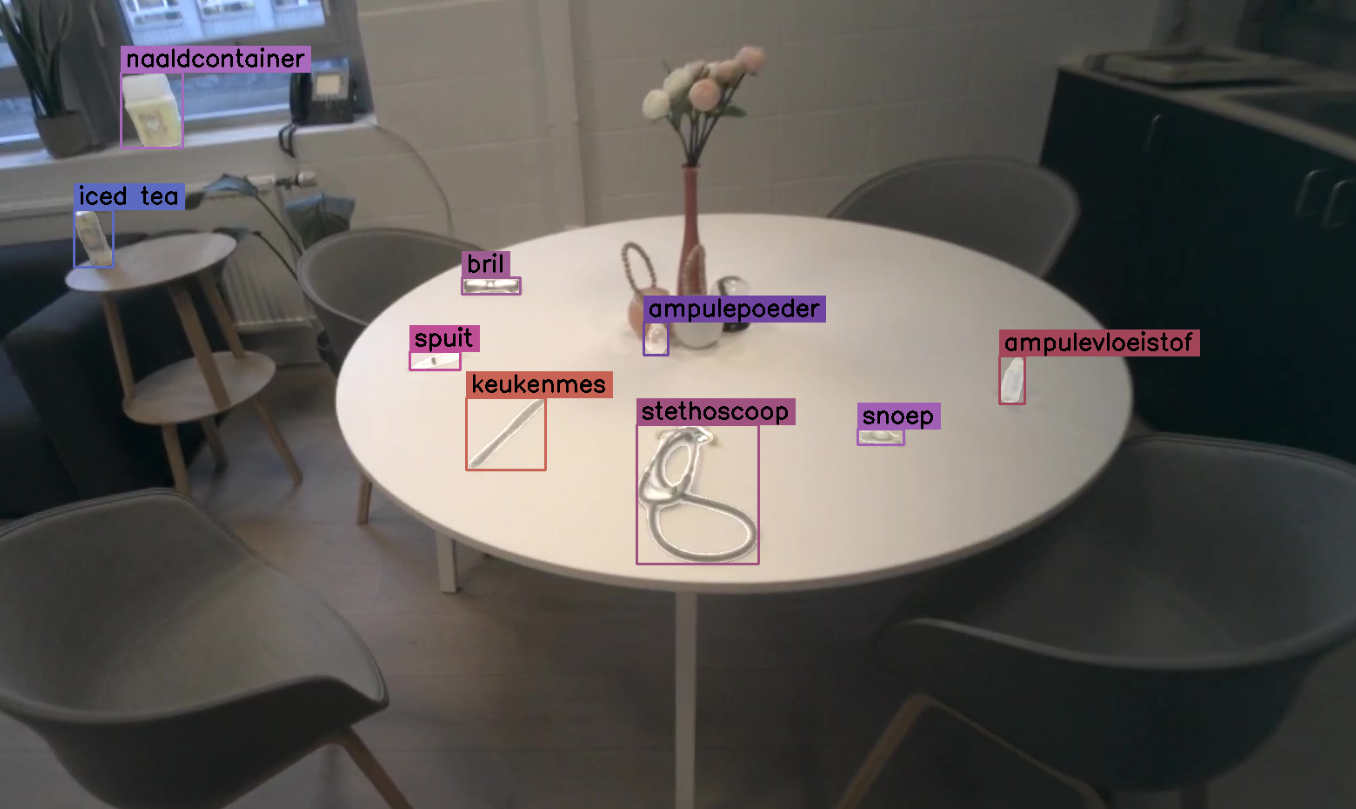
\includegraphics[width=0.8\textwidth]{objectdetection.png}
  \caption[]{\label{fig:object-detection}Voorbeeld van objectdetectie van verschillende objecten in een afbeelding.}
  \source{\url{https://djl.ai/examples/docs/object_detection.html}}
\end{figure}

\subsubsection{Van R-CNN naar Moderne Objectdetectiemodellen}

Een belangrijke doorbraak in objectdetectie kwam met de introductie van Region-based Convolutional Neural Networks (R-CNN) door \textcite{Girshick2014}.
R-CNN combineerde Convolutional Neural Networks (CNNs) met zogenaamde \textit{region proposals} om objecten nauwkeuriger te detecteren dan eerdere methoden.
Hoewel R-CNN goede prestatieverbeteringen liet zien, was het een traag algoritme dat moeilijk te trainen was. 
Dit kwam door de noodzaak om elke \textit{region proposal} afzonderlijk door een CNN te sturen, wat leidde tot een hoge rekentijd.
Om deze nadelen te overwinnen, werden verschillende verbeteringen geintroduceerd, waarvan de meest recente de You Only Look Once (YOLO) en Mask R-CNN modellen zijn.

\subsubsection{You Only Look Once (YOLO)}

You Only Look Once (YOLO), geïntroduceerd door \textcite{Redmon2016}, was een belangrijke stap vooruit binnen objectdetectie doordat het een veel eenvoudiger en sneller proces gebruikt. 
In plaats van afbeeldingen stap voor stap te analyseren zoals eerdere methoden (bijvoorbeeld Region-based Convolutional Neural Networks, R-CNN), verwerkt YOLO de gehele afbeelding tegelijkertijd in één analyse. 
Dit zorgt ervoor dat YOLO zeer snel objecten kan herkennen in \textit{real-time}, wat het ideaal maakt voor toepassingen waarbij snelheid belangrijk is.
Omdat YOLO de gehele afbeelding in één keer analyseert, wordt contextuele informatie zoals waar objecten zich bevinden tegenover elkaar, beter benut.
\newline \par
Toch heeft YOLO ook enkele nadelen. Het model heeft moeite met het detecteren van kleine en dicht opeengepakte objecten, wat kan leiden tot gemiste of overlappende detecties. 
Volgens onderzoek van \textcite{Huang2024} presteert YOLOv8 minder goed bij het detecteren van objecten kleiner dan 8x8 pixels. 
Dit komt doordat de standaard detectielaag van YOLO onvoldoende gedetailleerd is om kleine objecten nauwkeurig te detecteren. 
Hoewel optimalisaties zoals het toevoegen van extra detectielagen voor kleinere objecten verbeteringen bieden, blijft YOLO gevoelig voor problemen zoals overlappende en gemiste detecties bij dicht op elkaar geplaatste objecten.
\newline \par
Over de jaren heen zijn er verschillende versies van YOLO uitgebracht, waarvan de meest recente YOLOv11 is \autocite{Khanam2024}.
Deze modellen zijn beschikbaar via Ultralytics met een betaalde licentie\footnote{\url{https://www.ultralytics.com/license}} voor commercieel gebruik, maar zijn ook gratis beschikbaar voor open-source projecten en onderzoek.

\subsubsection{Mask R-CNN}

Mask Region-based Convolutional Neural Network (Mask R-CNN), geïntroduceerd door \textcite{He2018}, is een model dat niet alleen objecten detecteert met behulp van rechthoekige kaders (bounding boxes), 
maar ook precies aangeeft welke pixels bij elk gedetecteerd object horen. Dit gebeurt in twee stappen; eerst worden mogelijke objecten voorgesteld met zogenaamde \textit{region proposals}, en vervolgens
worden deze regio's verder geanalyseerd om drie zaken te bepalen. Ten eerste wordt de klasse van het object bepaald, ten tweede wordt de exacte locatie van het object bepaald met behulp van een bounding box, en ten laatste
wordt een masker gegenereerd dat aangeeft welke pixels bij het object horen. Het proces waarbij een masker wordt gegenereerd voor elk gedetecteerd object wordt \textit{instance segmentation} genoemd \autocite{Hafiz2020}.
Wanneer men ook een klasse toekent aan pixels in een afbeelding, wordt dit \textit{semantic segmentation} genoemd. Een laatste vorm van segmentatie is \textit{panoptic segmentation}, geintroduceerd door \textcite{Kirillov2019} waarbij zowel objecten als achtergrond worden geïdentificeerd.
Het verschil tussen deze vormen van segmentatie wordt geïllustreerd in figuur \ref{fig:segmentation}.

\begin{figure}[H]
  \centering
  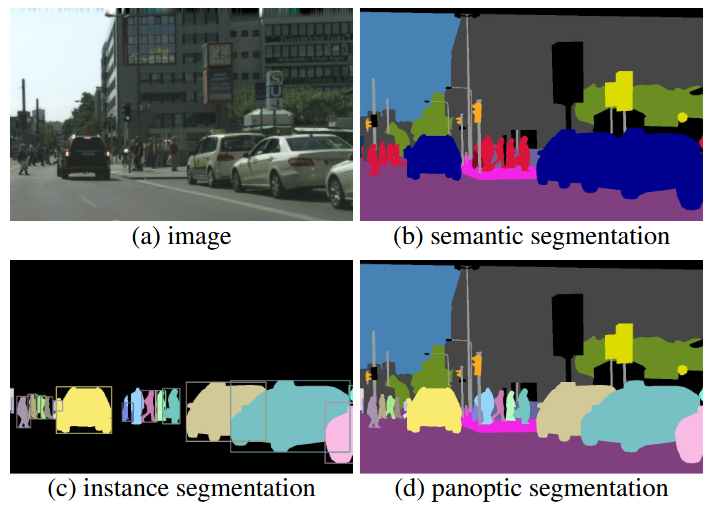
\includegraphics[width=0.8\textwidth]{segmentation.png}
  \caption[]{\label{fig:segmentation}Verschil tussen instance, semantic en panoptic segmentation \autocite{Kirillov2019}.}
\end{figure}

\subsection{Transformer-gebaseerde Objectdetectie}

Recentelijk zijn transformer-gebaseerde modellen in opkomst binnen Computer Vision als alternatief voor traditionele CNN-gebaseerde modellen, zoals YOLO en Mask R-CNN. 

\subsubsection{DETR}

Een belangrijk voorbeeld hiervan is DETR (DEtection TRansformer), geïntroduceerd door \textcite{Carion2020}.
\newline \par
Transformer-gebaseerde modellen zijn interessant vanwege hun vermogen om aandacht (attention) te richten op belangrijke delen van een afbeelding. 
Dit mechanisme stelt het model in staat om relaties tussen objecten en context beter te begrijpen.
Anders dan traditionele modellen gebruikt DETR geen vooraf bepaalde ankerpunten of zogenaamde `region proposals', om objecten te detecteren. 
In plaats daarvan behandelt DETR objectdetectie rechtstreeks als een voorspellingstaak, waarbij een afbeelding direct wordt verwerkt om objecten en hun locaties te identificeren.
Het DETR-model bestaat uit twee onderdelen: een \textit{encoder} en een \textit{decoder}. De encoder analyseert eerst de hele afbeelding om belangrijke kenmerken te onderscheiden en de context van de afbeelding te begrijpen. 
Vervolgens gebruikt de decoder specifieke `object queries' om de exacte locatie en de categorie van objecten te bepalen.
\newline \par
Een voordeel van DETR is dat het geen aparte stap nodig heeft om overlappende voorspellingen te verwijderen, hoewel dit soms in het beginstadium van voorspellingen wel nuttig kan zijn.
Toch heeft DETR ook enkele beperkingen. Zo presteert het model minder goed bij het detecteren van zeer kleine objecten door beperkte resolutie. 
Desondanks laat het model indrukwekkende resultaten zien in situaties die het tijdens training nog nooit heeft gezien, bijvoorbeeld wanneer er meerdere soortgelijke objecten in één afbeelding staan.
Opmerkelijk is dat DETR ook uitgebreid kan worden naar \textit{panoptic segmentation} taken.

\subsubsection{DINO}

Verder onderzoek door \textcite{Zhang2022} heeft geleid tot de ontwikkeling van DINO (DETR with Improved DeNoising anchOr boxes). 
DINO bouwt voort op DETR door onder andere verbeterde denoising-technieken tijdens training te gebruiken, wat resulteert in nauwkeurigere detecties. 
Dit wordt bereikt door het gebruik van zowel positieve als negatieve voorbeelden om verwarring tussen overlappende voorspellingen te verminderen. 
Daarnaast gebruikt DINO een query-selectiemethode die positie-informatie uit de encoder gebruikt om de initiële voorspellingen (\textit{queries}) van de decoder beter te initialiseren. 
Ten slotte introduceert DINO een \textit{look forward twice}-techniek, waarbij voorspellingen uit latere decoderlagen worden gebruikt om eerdere voorspellingen verder te verbeteren. 
Deze innovaties zorgen ervoor dat DINO aanzienlijk beter presteert dan eerdere DETR-gebaseerde modellen.

\subsubsection{Grounding DINO}

In 2023 introduceerde \textcite{Liu2023} Grounding DINO, een uitbreiding op DINO gericht op \textit{open-set objectdetectie}. Dit houdt in dat het model objecten kan detecteren die tijdens de training niet expliciet zijn aangeleerd. 
Grounding DINO integreert taalbegrip met visuele detectie, waardoor het mogelijk wordt om objecten op basis van natuurlijke taal te identificeren en te lokaliseren.
\newline \par
Visuele kenmerken uit een afbeelding worden gecombineerd met taalkundige informatie uit teksten, zoals categorieën of beschrijvende zinnen. 
Dit gebeurt via een \textit{feature enhancer}, die beeld- en tekstinformatie samenbrengt, en een taalgestuurde query-selectiemethode, waarmee relevante beeldgebieden worden geselecteerd op basis van tekstuele input. 
Vervolgens gebruikt het model een \textit{cross-modality decoder}, waarin informatie uit beide modaliteiten verder gecombineerd wordt voor nauwkeurigere detecties.
\newline \par
Het model wordt getraind op grootschalige datasets, bestaande uit foto's met bijbehorende beschrijvingen en labels. 
Hierdoor leert Grounding DINO generaliseren naar nieuwe, niet eerder getoonde objecten. Dit stelt het model in staat om, zonder verdere training, objecten te herkennen uit tekstuele beschrijvingen die het nog nooit eerder heeft gezien.
\newline \par
Hoewel de resultaten van Grounding DINO veelbelovend zijn, is het model niet geschikt voor real-time toepassingen, of toepassingen waarbij heel veel afbeeldingen moeten worden verwerkt \autocite{Son2024}.
Omdat het model gebaseerd is op een transformer-architectuur, en het veel klassen moet kunnen detecteren waardoor het een groot model is, presteert het meer dan 30 keer trager in vergelijking met YOLO modellen.

\subsection{Segmentatie}

In de voorgaande sectie hebben we reeds gesproken over verschillende vormen van segmentatie, zoals instance, semantic en panoptic segmentation.
Vaak zijn de taken van objectdetectie en segmentatie nauw met elkaar verbonden, aangezien beide taken objecten in een afbeelding lokaliseren en classificeren.
Toch willen we in deze sectie dieper ingaan op een aantal modellen die specifiek gericht zijn op segmentatie, met een oog voor voorgetrainde modellen die geen verdere training vereisen.

\subsubsection{Meta Segment Anything Model (SAM)}

In 2023 introduceerde Meta het open-source Segment Anything Model (SAM), een model ontworpen om objecten in afbeeldingen te segmenteren op basis van gebruikersinput, ook wel prompts genoemd \autocite{Kirillov2023}. 
Het doel van SAM is om flexibele en veelzijdige segmentatie mogelijk te maken, waarbij gebruikers eenvoudig kunnen aangeven welke delen van een afbeelding ze willen segmenteren via punten, 
rechthoeken, maskers of zelfs korte tekstuele beschrijvingen. Dit wordt het `promptable segmentation'-principe genoemd.
\newline \par
SAM bestaat uit drie belangrijke onderdelen: een beeldencoder, een promptencoder en een masker-decoder. 
De beeldencoder verwerkt de afbeelding één keer en creëert een zogenoemde image embedding, een compacte representatie van de afbeelding waarin belangrijke kenmerken zijn opgeslagen. 
Vervolgens wordt de prompt (zoals een punt of rechthoek) verwerkt door de promptencoder en gecombineerd met de representatie uit de beeldencoder. 
De masker-decoder gebruikt vervolgens deze gecombineerde informatie om het uiteindelijke masker te genereren dat het gewenste object nauwkeurig identificeert.
\newline \par
Een opvallend aspect van SAM is het vermogen om ambiguïteit te herkennen en daarmee om te gaan. 
Wanneer één prompt meerdere mogelijke interpretaties heeft, bijvoorbeeld een punt dat zowel naar een persoon als een kledingstuk verwijst, kan SAM meerdere segmentatiemaskers genereren die elk een mogelijke interpretatie weergeven. 
Vervolgens wordt voor elk masker een betrouwbaarheidswaarde berekend, waarmee het model aangeeft welk masker het meest waarschijnlijk overeenkomt met de intentie van de gebruiker.
\newline \par
De kracht van SAM ligt in zijn brede toepasbaarheid zonder dat verdere training vereist is (zero-shot generalisatie). 
Dit betekent dat SAM in staat is om direct te worden ingezet voor nieuwe beelden en taken die het nog niet eerder heeft gezien, wat erg nuttig is voor interactieve toepassingen en snelle analyses.
Hoewel SAM indrukwekkende resultaten levert en een grote stap vooruit betekent voor segmentatiemodellen, heeft het ook enkele beperkingen. 
De belangrijkste is dat het model, hoewel snel genoeg voor interactieve toepassingen, minder geschikt is voor real-time toepassingen met zeer hoge snelheden zoals videostreaming, vanwege de benodigde rekencapaciteit voor de beeldverwerking.
\newline \par
Het jaar nadien werd een verbeterde versie van het model uitgebracht, SAM 2 \autocite{Ravi2024}. 
SAM 2 voegt belangrijke verbeteringen toe, zoals een uitbreiding naar videosegmentatie met behulp van een geheugenmodule, waardoor het model eerdere prompts en segmentaties kan onthouden en toepassen op opeenvolgende videoframes. 
Dit maakt SAM2 heel interessant voor de toepassingen binnen het Zorglab, waarbij het volgen van objecten doorheen de video een belangrijke rol kan spelen.
Daarnaast is SAM 2 ongeveer zes keer sneller bij het segmenteren van afbeeldingen dan het oorspronkelijke SAM-model, wat het geschikt maakt voor een bredere reeks real-time toepassingen.

\subsubsection{FastSAM}

Zou het kunnen dat SAM nog sneller kan? 
Dat is precies wat \textcite{Zhao2023} zich afvroegen bij het ontwikkelen van FastSAM, een verbeterde versie van SAM die tot 50 keer sneller is dan het originele model, zonder veel in te boeten aan nauwkeurigheid.
FastSAM bereikt dit door het segmentatieproces op te splitsen in twee opeenvolgende stappen: het segmenteren van alle objecten in een afbeelding en vervolgens het selecteren van specifieke objecten aan de hand van een gebruikersprompt.
\newline \par
In de eerste fase, genaamd \textit{all-instance segmentation}, maakt FastSAM gebruik van een CNN gebaseerd op het YOLOv8-seg model, een objectdetector met een speciale tak voor \textit{instance segmentation}. 
De tweede fase, de \textit{prompt-guided selection}, gebruikt vervolgens de gegenereerde segmentatiemaskers uit de eerste fase en selecteert specifiek het gewenste gebied op basis van verschillende prompts. 
Deze prompts kunnen bestaan uit punten (\textit{point prompts}), rechthoeken (\textit{box prompts}) of zelfs tekstuele beschrijvingen (\textit{text prompts}). 
Bij een punt-prompt wordt bijvoorbeeld gekeken welk segmentatiemasker het opgegeven punt bevat, terwijl een box-prompt gebruikmaakt van de overlap tussen een opgegeven rechthoek en bestaande segmentatiemaskers.
Zo kunnen we bij eye-tracking data bijvoorbeeld een punt-prompt gebruiken op basis van de blikrichting van de gebruiker om objecten te selecteren uit een all-instance segmentatie.
Merk op dat hier geen klassen worden toegewezen aan objecten, enkel de segmentatie van objecten wordt bepaald. 
Daarom zullen segmentatiemodellen zoals FastSAM en SAM moeten worden gecombineerd met objectdetectiemodellen om na te gaan welke objecten er in de afbeelding aanwezig zijn.
\newline \par
FastSAM is beschikbaar in de Model Hub van Ultralytics\footnote{\url{https://docs.ultralytics.com/models/fast-sam/}} en kan gratis worden gebruikt voor open-source projecten en onderzoek.

\subsection{Image Embedding}

Naast objectdetectie en segmentatie speelt ook image embedding een steeds belangrijkere rol binnen Computer Vision. 
Image embedding is een techniek waarbij afbeeldingen worden omgezet naar numerieke vectoren, ook wel feature vectors genoemd. 
Deze vectoren zijn eigenlijk een reeks getallen die belangrijke visuele kenmerken en eigenschappen van een afbeelding beschrijven. 
Ze kunnen worden beschouwd als een compacte, numerieke `vingerafdruk' van een afbeelding, waarbij visueel vergelijkbare afbeeldingen corresponderen met vectoren die dicht bij elkaar liggen in de hoog-dimensionale ruimte.
Enkele voorbeelden van de mogelijkheden van image embeddings zijn te zien in figuur \ref{fig:dinov2}.
\newline \par
Deze techniek is vooral interessant voor toepassingen waarbij men op een efficiënte manier wil bepalen om welk object het gaat, zonder hiervoor telkens nieuwe detectiemodellen te moeten trainen. 
Wanneer een selectie van objecten via segmentatie (zoals met SAM) gedetecteerd wordt, kan een image embedding gebruikt worden om automatisch te bepalen om welk specifiek object het gaat. 
Dit gebeurt door de gegenereerde vector van het gedetecteerde object te vergelijken met een vooraf opgebouwde database van bekende objecten. 
Het gebruik van image embeddings biedt een aantal voordelen: het is robuust tegen variaties in belichting, perspectief, en andere visuele veranderingen, waardoor het model goed blijft presteren, zelfs wanneer objecten er anders uitzien dan tijdens de training.

\subsubsection{CLIP}

Een van de eerdere modellen die image embeddings populair maakten is CLIP (Contrastive Language-Image Pre-training), geïntroduceerd door OpenAI in 2021 \autocite{Radford2021}.
CLIP koppelt tekstuele beschrijvingen aan afbeeldingen tijdens de training, waardoor het model leert om afbeeldingen en teksten in dezelfde vectorruimte te plaatsen. 
Dit betekent dat afbeeldingen niet alleen herkend kunnen worden op basis van visuele kenmerken, maar ook gekoppeld kunnen worden aan tekstuele beschrijvingen zonder dat hiervoor expliciete labels nodig zijn.

\subsubsection{DINOv2}

DINOv2, geïntroduceerd in 2024 door \textcite{Oquab2024}, bouwt voort op eerdere modellen zoals DETR en DINO, met verbeteringen in nauwkeurigheid en toepasbaarheid zonder extra finetuning. 
Net zoals eerdere embedding-modellen genereert DINOv2 numerieke representaties van afbeeldingen, maar onderscheidt zich door een sterk verbeterde generalisatiekracht. 
Dit betekent dat het model beter in staat is om nieuwe objecten en situaties te herkennen zonder verdere training.
\newline \par
DINOv2 is gebaseerd op transformer-architecturen en maakt gebruik van self-supervised learning (SSL). 
Hierbij leert het model zelfstandig relevante kenmerken van afbeeldingen zonder gebruik te maken van expliciete labels. 
In tegenstelling tot veel eerdere modellen presteert DINOv2 zowel goed op algemene taken, zoals het herkennen van categorieën van objecten (auto's of vliegtuigen), als op taken waarbij het exacte exemplaar (een specifiek gebouw of schilderij) geïdentificeerd moet worden. 
\newline \par
Daarnaast biedt DINOv2 ook goede prestaties bij segmentatietaken. Door een eenvoudige lineaire laag aan het model toe te voegen, kunnen zeer goede segmentatiemaps worden gegenereerd zonder verdere optimalisatie of training van het volledige model. 
Met name bij gebruik van zogenaamde multiscale augmentaties (waarbij het model de afbeelding op meerdere resoluties analyseert), 
behaalt DINOv2 segmentatieprestaties die vergelijkbaar zijn met gespecialiseerde segmentatiemodellen zoals SAM en FastSAM.

\begin{figure}[H]
  \centering
  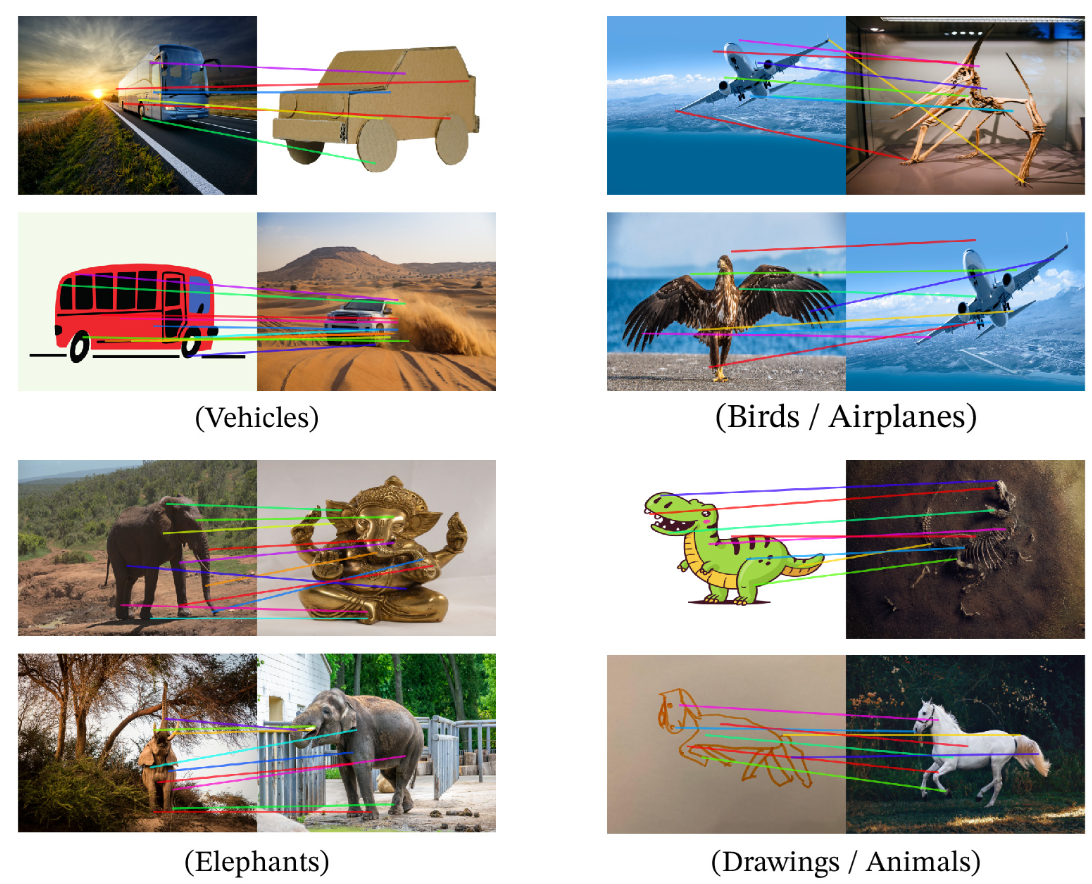
\includegraphics[width=0.8\textwidth]{dinov2.png}
  \caption[]{\label{fig:dinov2}Enkele voorbeelden van de mogelijkheden van DINOv2 image embeddings \autocite{Oquab2024}.}
\end{figure}

\section{Eyetracking en Computer Vision}

Ten slotte is het interessant om stil te staan bij recente implementaties van Computer Vision in combinatie met eyetracking-technologie.
\newline \par
In 2023 onderzochten \textcite{CederinBremberg2023} de mogelijkheden van bestaande computer vision modellen om automatisch te detecteren welke objecten een gebruiker bekijkt tijdens een eyetracking-sessie.
Net zoals deze bachelorproef gebruikten ze de Tobii Pro Glasses 3, wat hun onderzoek interessant maakt als referentie voor het omgaan met de eyetracking data van deze specifieke bril.
Een probleem bij hoofd-gemonteerde eyetrackers is dat er vaak bewegingsruis aanwezig is, zeker als het hoofd van de gebruiker veel beweegt. Dit maakt het toepassen van computer vision modellen moeilijker.
In hun onderzoek vergeleken ze twee ruisreductiemodellen, namelijk Restormer en DeblurGAN-v2, om de kwaliteit van de eyetracking data te verbeteren. Ze concludeerden dat DeblurGAN-v2 betere resultaten opleverde dan Restormer.
Ook onderzochten ze de prestatieverschillen tussen YOLOv8 en DINO modellen op de eyetracking data. Uit hun resultaten blijkt dat DINO beter presteert dan YOLOv8 in elk testscenario. Ze concludeerden echter ook dat 
DINO modellen een langere rekentijd nodig hebben dan de YOLO modellen.
\newline \par
SAM werd ook onderzocht in combinatie met eyetracking data door \textcite{Wang2023} in hun applicatie genaamd `GazeSAM'. Dit onderzoek richtte zich op het segmenteren van de objecten waarnaar de gebruiker kijkt tijdens een eyetracking-sessie.
Een belangrijk onderschijd tussen de context van dit onderzoek en deze bachelorproef is dat er gebruik gemaakt werd van screen-based eyetracking, waarbij de gebruiker naar een computerscherm keek in plaats van een fysieke omgeving.
De blikrichting van de gebruiker werd gebruikt als basis voor een punt-prompt, waarmee SAM de objecten in de afbeelding kon segmenteren. Het bleek dat SAM soms moeilijkheden had met het segmenteren van medische afbeeldingen, omdat 
SAM voornamelijk getraind is op alledaagse objecten. Dit zal echter geen probleem vormen voor de toepassingen binnen het Zorglab, waar de objecten voornamelijk alledaagse objecten zijn. Een ander nadeel van SAM was dat het model 
moeilijkheden had met het correct segmenteren van objecten op basis van een enkele punt-prompt, waardoor verdere manuele interventie nodig was.